\section{Sprint 1}
As stated above the first sprint was focused on reducing the overhead of future development by removing unnecessary and excessive factors of the  initial proof of concept, namely the authorization system Auth0 and the front end state management control redux js. The product owner and I deemed this an important step to reduce waste at later stages of development and not build up technical overhead.

\subsection{Auth0}
Auth0 is a third party single sign on and token based authentication system that the initial proof of concept was using for user authentication. While this was easy to setup and manage, it was not a suitable long term solution due to extra costs incurred through licensing and extra latency of  relying on a third party service instead of having the authentication handled by the same service as the Restful API. Auth0 would potentially be able to provide better security of data and more complex 
After some consideration we decided it was best to replace the authentication with a JSON web token (JWT) system as it is industry standard for `URL-safe means of representing claims to be transferred between two parties'\cite{jones2015rfc}.

\subsection{JWT Tokens}
JSON web tokens consist of an encrypted token that contains a payload consisting of a JSON object and is encrypted via a JSON web signature. Using these JWT tokens we are able to securely authenticate users and produce a token for them that tells the API their user role, organisation, id and creation date. This allows them to stay logged in securely and helps govern access to the API based on their role.

\subsection{Redux JS}
Redux is a state container for JavaScript applications, it was used to keep the current state of the front end under control to help lower load times and preserve data and scope. Redux is a great tool for managing your app state in a way that allows states to persist through the same session or even through sessions if saved locally. However it comes with some trade offs and requires you to structure your apps data in certain ways:

\begin{itemize}
\item State needs to be described as plain JSON objects and arrays.
\item Describe changes in the system as plain objects
\item Any logic for handling changes to the state needs to be as pure functions
\end{itemize}

These requirements for how you structure logic, state and changes within the system make sense and are often good practices to follow if you wish for your code to be decouple what happened, for example a button press or data finish loading with how this changes things, for example when the data is loaded change the values on screen. However because of the relatively simple states required for this web application and no foreseeable need for a persistent state. It was decided that maintaining the state store through Redux was not required and the app.

So for this sprint the main focus was removing these unnecessary libraries and replace them with current solutions. The Auth0 authentication service was replaced with our own JWT focused authentication using and redux state management was replaced with logic within the components.

\subsection{Summary}
With this sprint focused on removing some of the system that were no longer required a lot of this sprint went into refactoring the code base and implementing the new authentication system. The refactoring of removing redux from the system included moving the action logic for components into the components themselves. This reduced the indirection within the code but more tightly couples the components with the logic and actions of the system. This means that it is harder to implement another component with very similar features that should act the same way but with a different look or display. This was considered a reasonable trade off as it simplifies the workflow of each action and makes the code easier to follow, because the products logic flow should be reasonably simple with no overly complex actions or components.


 \begin{figure}
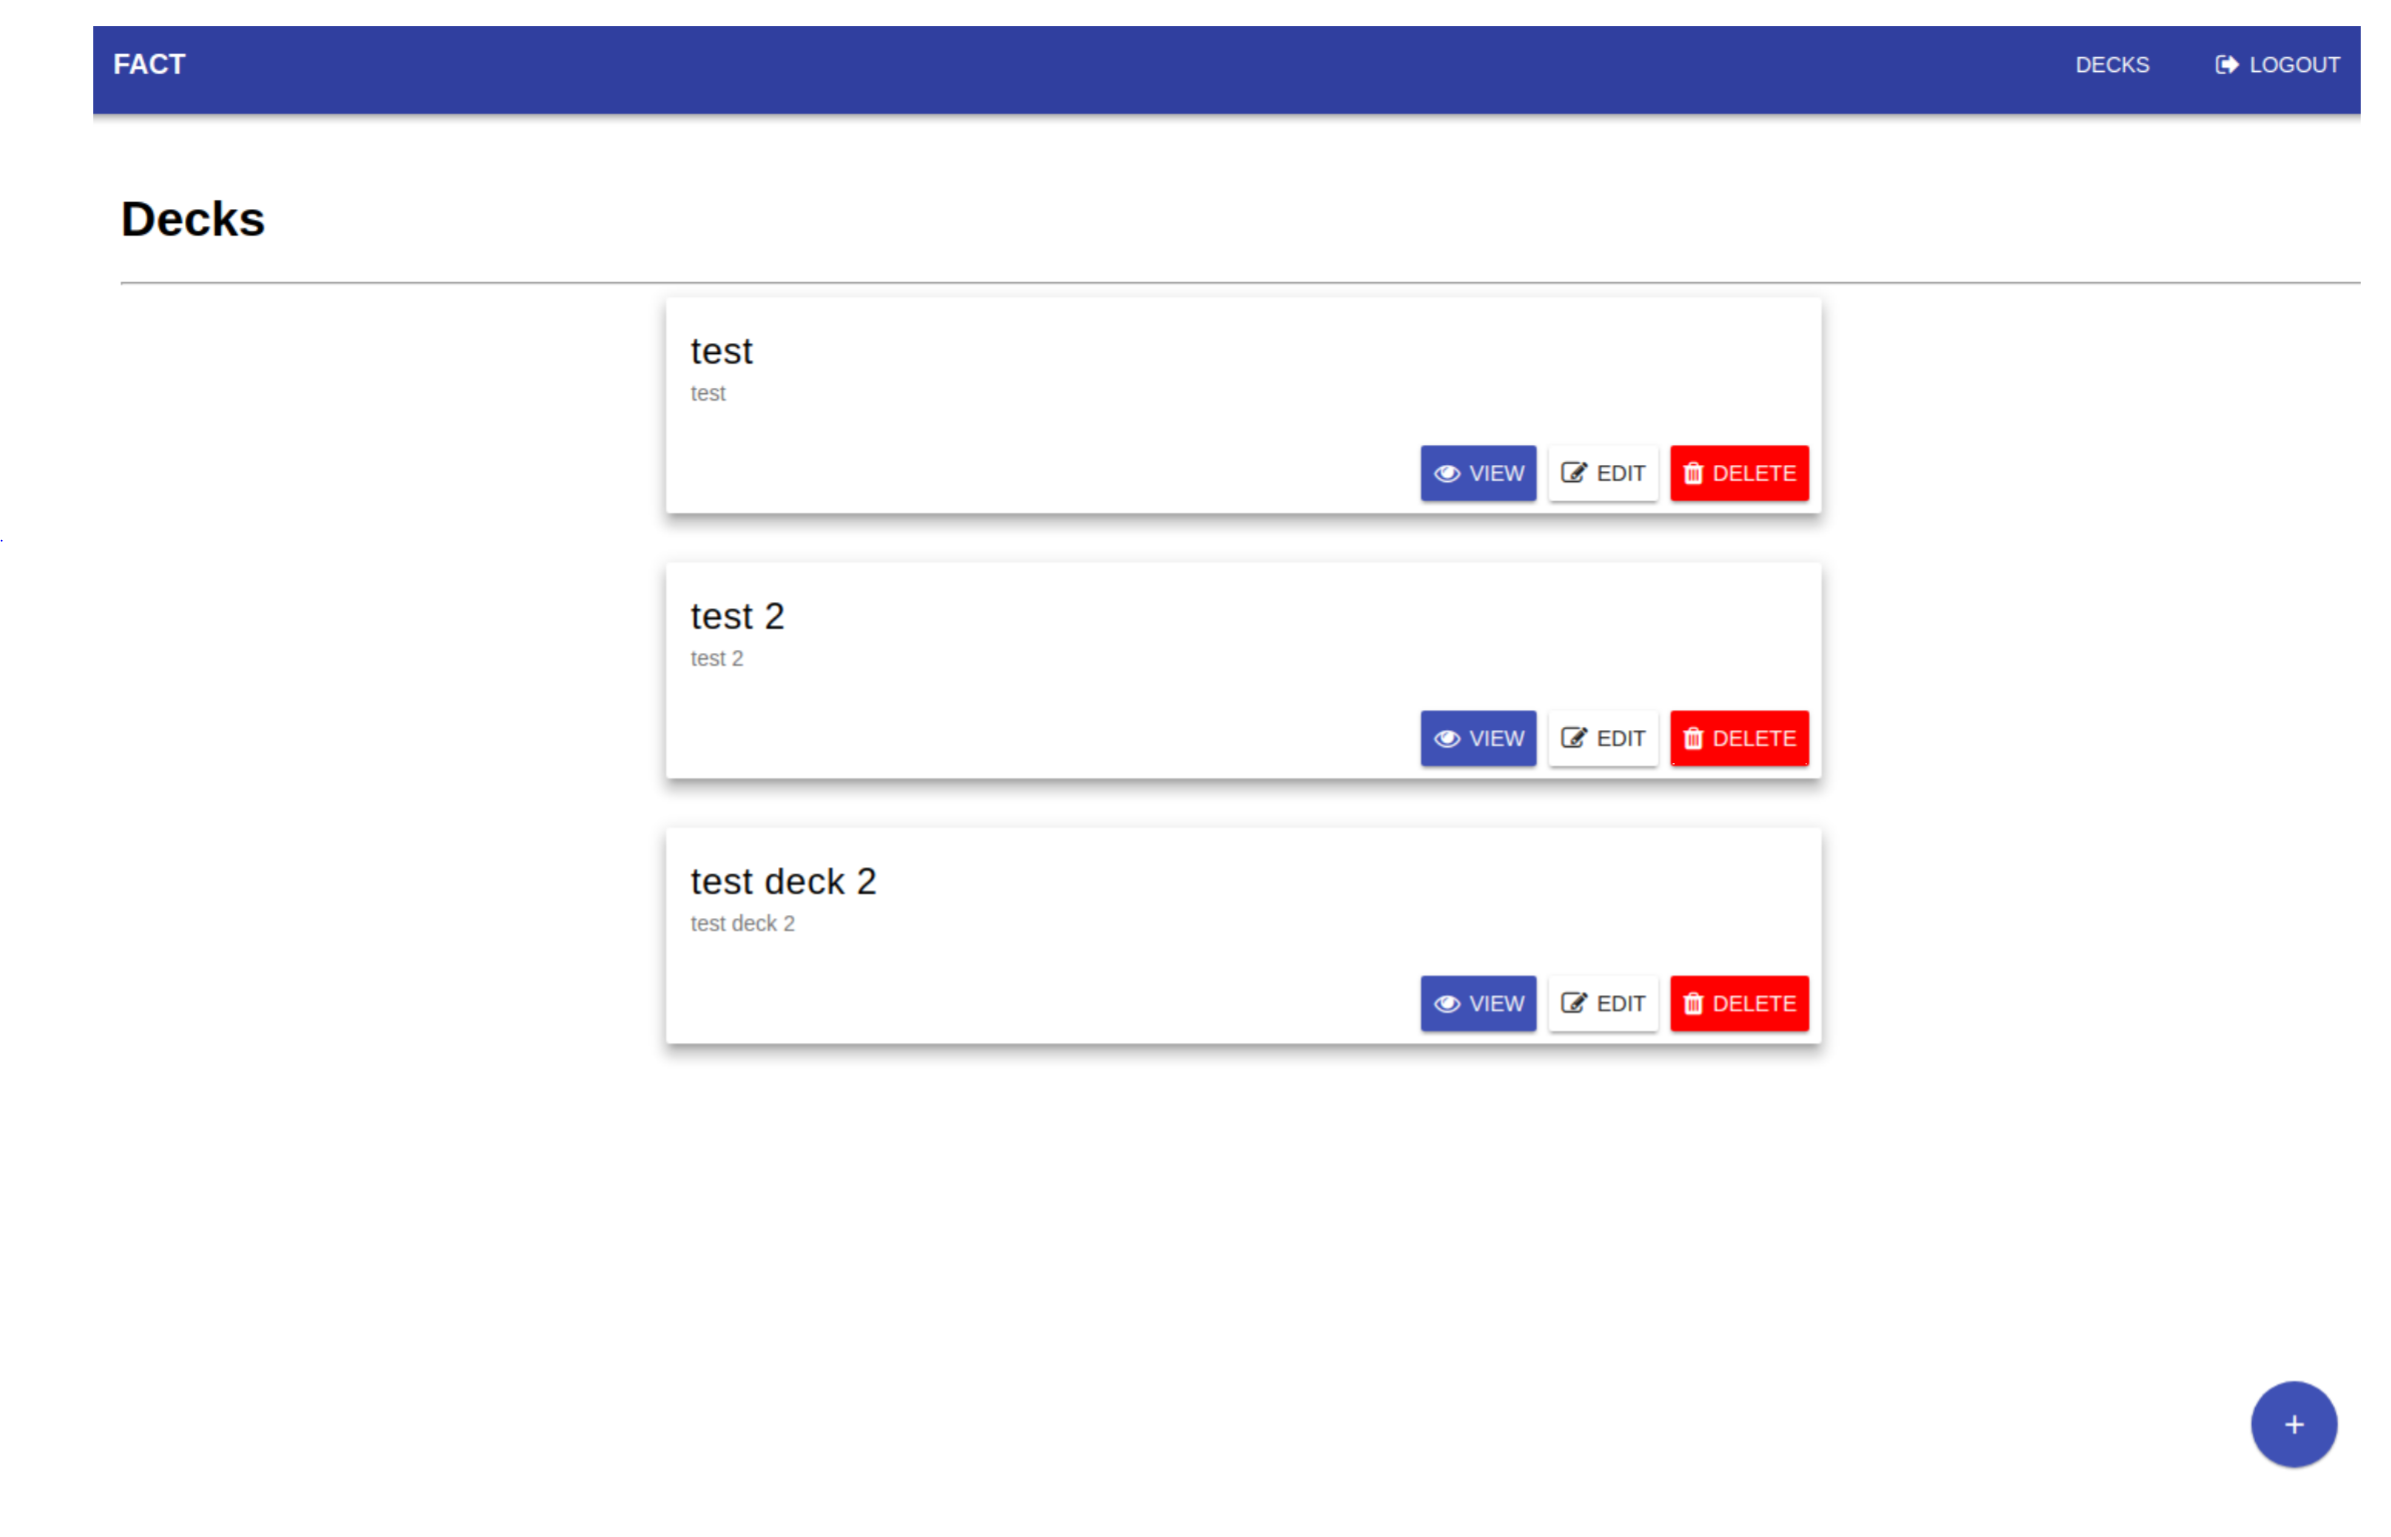
\includegraphics[width=\textwidth]{s1}
\caption{Display of a fact deck after development in sprint 1}
\centering
\end{figure}
